\documentclass{article}
\usepackage[pdfcreator={LaTeX}]{hyperref}
\usepackage{graphicx}
\usepackage[utf8]{inputenc} 
\usepackage[ngerman]{babel}


\usepackage{tikz}
\usetikzlibrary{arrows,shadows}
\usepackage{pgf-umlsd}


\begin{document}
\begin{titlepage}

\begin{center}
\textbf{\textsc{\LARGE Entwurf}}

{\large \today}

\vspace{2cm}
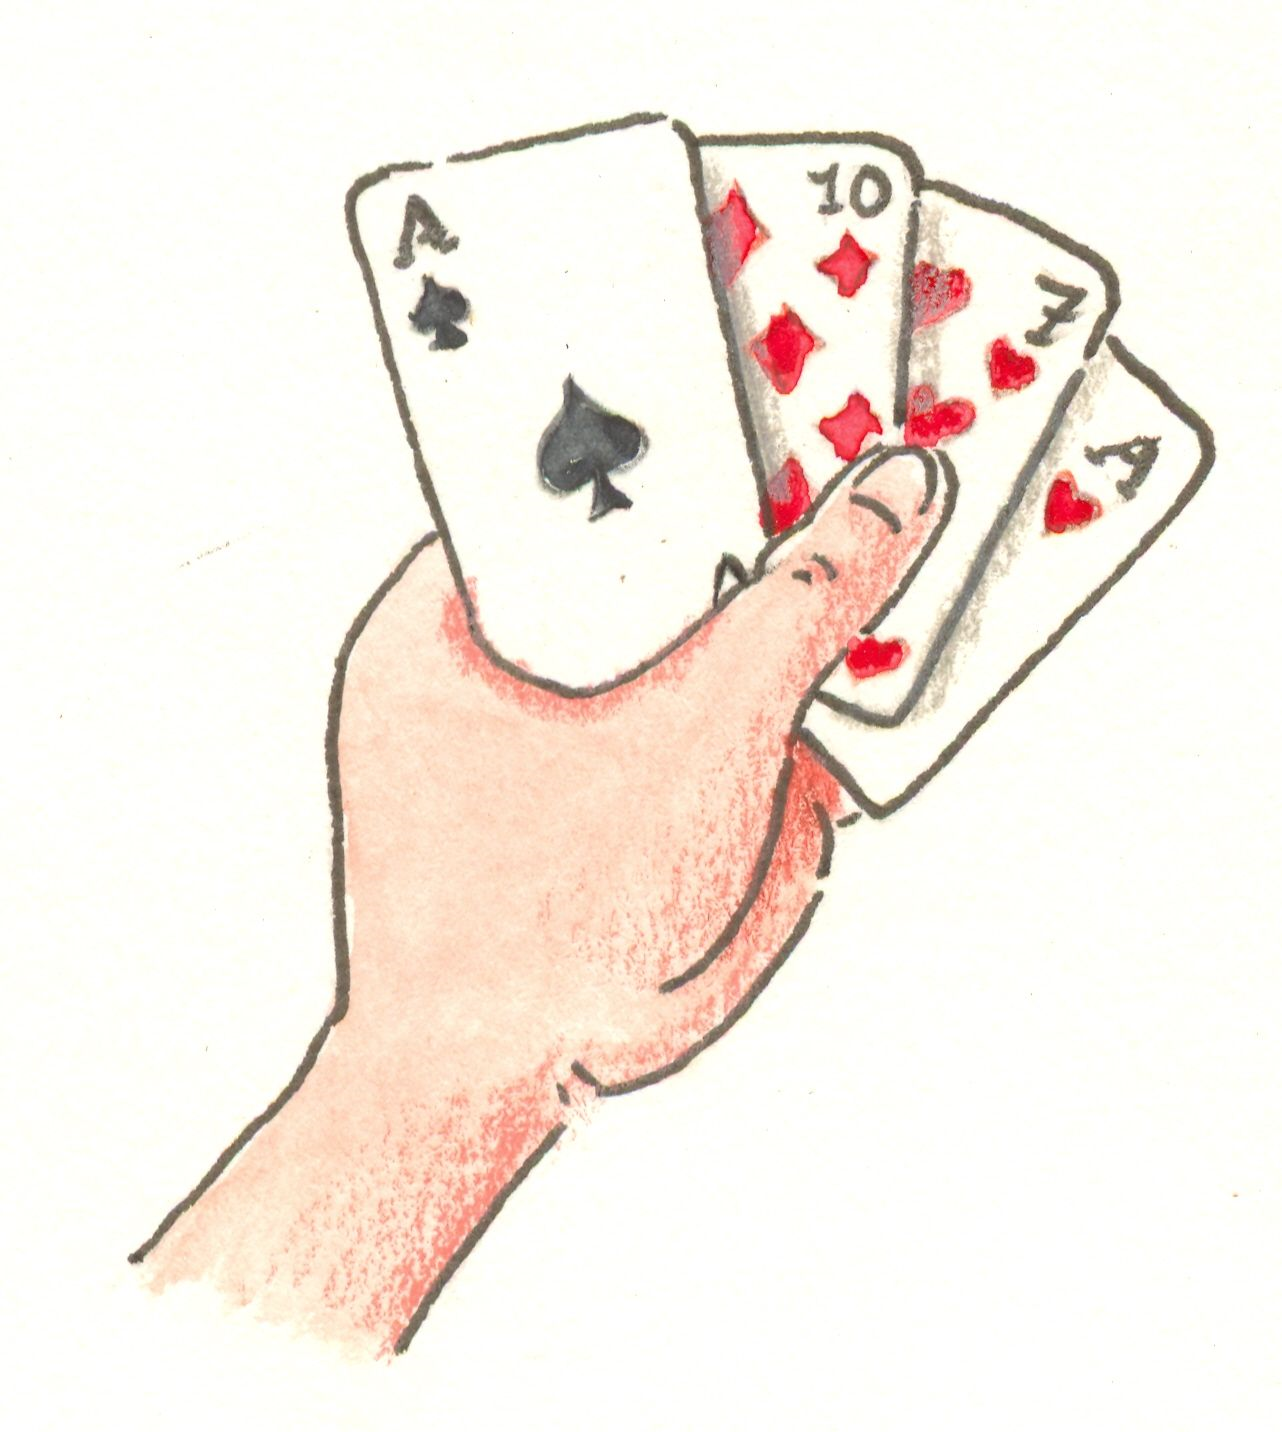
\includegraphics{kartenspiel}
\ \\
\ \\

\textbf{\textsc{\LARGE NET-WizHearts}}
\vspace{2cm}

\begin{tabular}{|c|c|c|}\hline
   Phase & Verantwortlicher & E-Mail \\ \hline\hline
   Pflichtenheft & Alina Meixl &  alina@meixl.de \\ \hline
   Entwurf & Viktoria Witka & witkaviktoria@freenet.de \\ \hline
   Spezifikation & Daniel Riedl & dariedl14@yahoo.de \\ \hline
   Implementation & Andreas Altenbuchner& a.andi007@gmail.com\\ \hline
   Verifikation & Patrick Kubin & kubin@fim.uni-passau.de\\ \hline
   Präsentation & w& w\\ \hline
 \end{tabular}

\end{center}

\end{titlepage}

\tableofcontents
\newpage

\section{Einleitung}
In diesem Dokument wird der konzeptionelle Entwurf des Online Multiplayer Kartenspiels NET-WizHearts dargestellt.\\
\ \\
Das Architektur-Diagramm verdeutlicht die Kommunikation zwischen Server und Client, die für die Anwendung von großer 
Bedeutung ist. Des Weiteren wird die Nutzung eines Regelwerkes veranschaulicht.\\
\ \\
Durch Angabe der Klassenstruktur wird eine erste Übersicht über die verschiedenen Komponenten des MVC-
Modells, welches der Anwendung zugrunde liegt, gegeben. Zu Illustrationszwecken werden außerdem einzelne Funktionsaufrufe
beispielhaft in Sequenzdiagrammen dargestellt.\\
\ \\
Durch das Verwenden des MVC Design Patterns wird eine Unabhängigkeit der View-Schicht 
vom restlichen System erzielt, so dass die graphische Oberfläche ohne Anpassung 
der Modell- und Controllerschicht auch für andere Regelwerke einsetzbar ist. Die Nutzung des Observer-Patterns erleichtert zudem
die Kommunikation zwischen der Modell- und View-Schicht.\\
\  \\



\section{Architektur-Diagramm}
Client-Server Diagramm. Der Client hat MVC Architektur.
\  \\
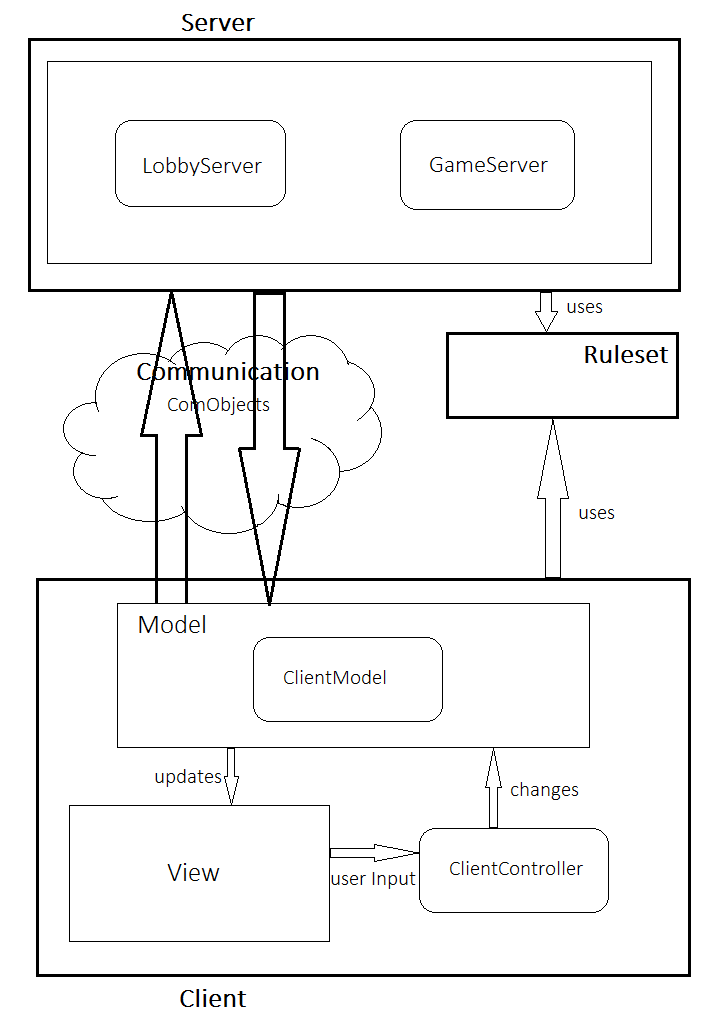
\includegraphics[height=15cm]{ArchitekturDiagramm}
\newpage
\section{Klassendiagramm}

\subsection{Packages}
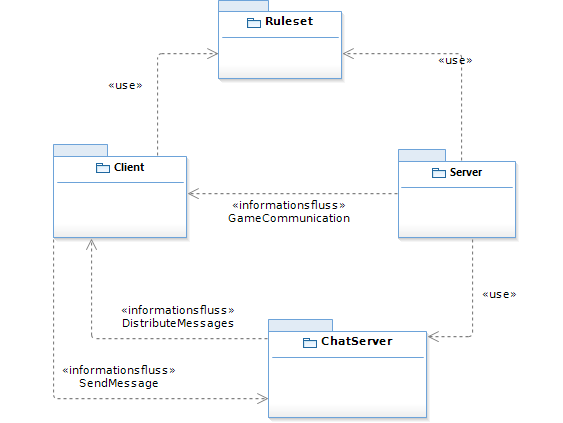
\includegraphics[width=\textwidth]{Packages}

\subsection{Server}
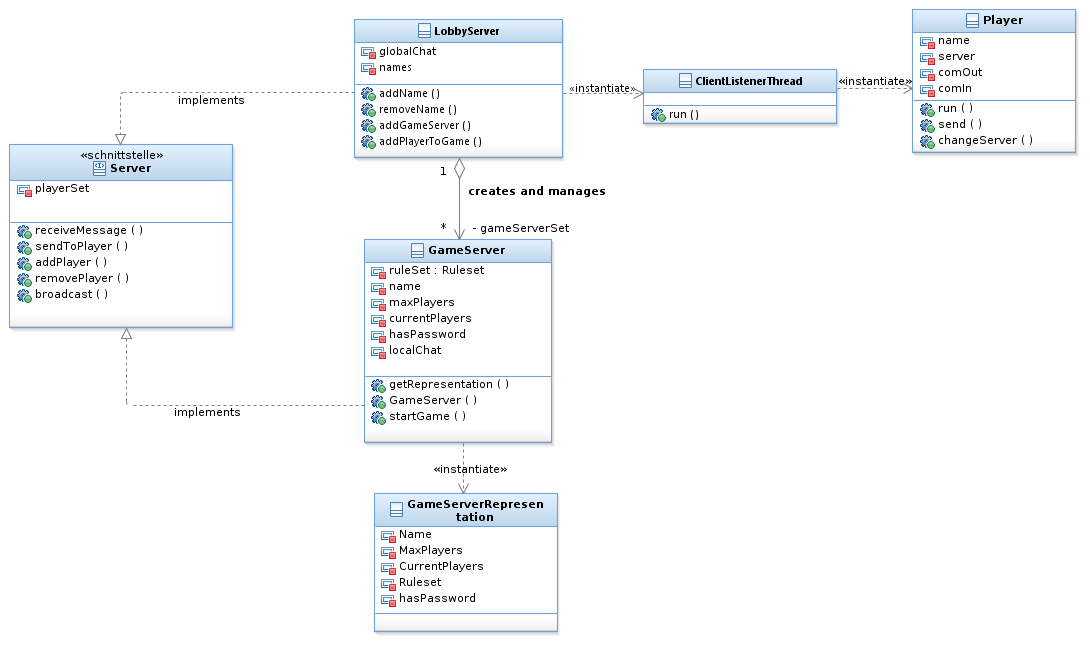
\includegraphics[width=\textwidth]{Server}
\textbf{ServerMain} ist die Hauptklasse des Servers, welche Konfiguration und Wartung des Servers implementiert. \\
		\textbf{Schnittstelle Server} liefert einen Satz von Methoden, die von der LobbyServer-Klasse und der GameServer-Klasse implementiert werden. \\
		Mit receiveMessage() kann eine Playerinstanz ein ComObjekt an eine Serverinstanz zur weiteren Verarbeitung weiterleiten. \\
		Mit sendToPlayer() kann eine Serverinstanz ein ComObjekt an eine Playerinstanz weiterreichen. \\
		Sammelaufrufe werden durch die broadCast() Methode implementiert.
		\textbf{LobbyServer} erstellt neue Spiele (/F126/) und ist sowohl für die Verwaltung aller Spiele (/L110/), als auch die der Spieler in der Lobby zuständig (/L100/). Die LobbyServer-Klasse implementiert die Server-Schnittstelle. Über die Methode addGameServer() wird ein Spiel erstellt (/L300/) und addPlayerToGame() fügt Spieler den bestehenden Spielen hinzu. Es werden auflaufenden ComObjekte anhand ihrer Klasse weiter verarbeitet und steuern so die Belange der Lobby. \\
		\textbf{ClientListenerThread} akzeptiert eingehende TCP-Verbindungen und erstellt die Instanzen der Klasse Player. \\
		\textbf{GameServer} verwaltet ein Spiel, dessen Spieler, sowie den Chatroom im Spiel (/L260/). Der GameServer leitet Aufrufe vom Regelwerk an die betreffenden Spieler weiter. Die GameServer-Klasse implementiert die Server-Schnittstelle. Über den Methodenaufruf startGame() können Spiele vom Spielleiter gestartet werden. Es werden auflaufende ComObjekte anhand ihrer Klasse weiter verarbeitet und steuern so die Belange des Spieles.\\
		\textbf{Player} repräsentiert einen Client, enthält den Namen des Clients und verwaltet die Ein- und Ausgänge seiner Socketverbindung. Send() ermöglicht es Serverinstanzen-ComObjekte an den Client zu senden. \\

\subsection{Client}
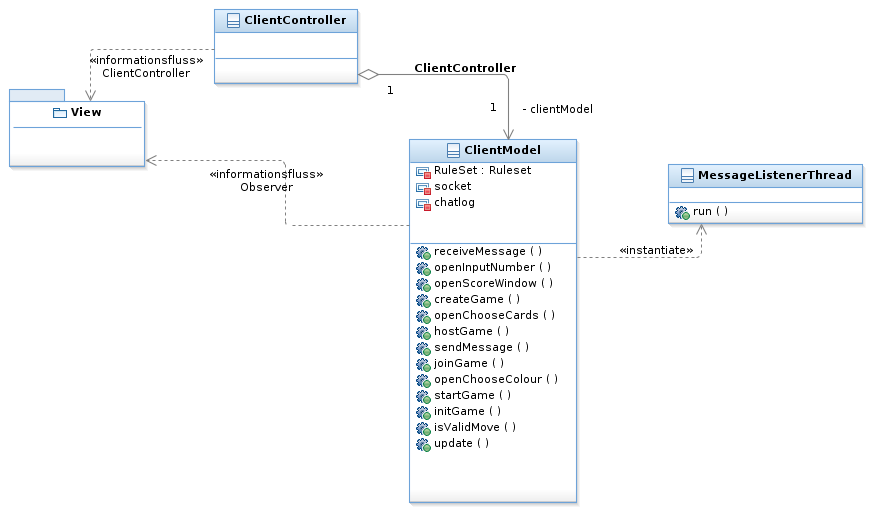
\includegraphics[width=\textwidth]{Client}
\textbf{ClientMain}: Dies ist die Hauptklasse des Clients, die beim Starten des Programmes ausgeführt wird. Sie erzeugt ein neues ClientController Objekt.\\

\textbf{ClientController}: Diese Klasse ist für die Kommunikaton zwischen dem ClientModel und dem ClientController zuständig.\\
Sobald der ClientController von der ClientMain Klasse erzeugt wird, erzeugt dieser wiederum das ClientModel und die ClientView, wobei zunächst nur die Login Klasse sichtbar ist. Der ClientController enthält alle ActionListener der View und leitet durch diese Benutzereingaben an das ClientModel weiter.\\

\textbf{ClientModel} [erbt von Observable]: Das ClientModel ist die Schnittstelle zwischen dem MessageListenerThread, dem Ruleset und der View.\\ 
Das Model prüft Nachrichten, welche es vom MessageListenerThread über die Methode receiveMessage() bekommt .Je nach 'command' des übergebenen ComObjects leitet es das ComObject an das Regelwerk weiter, oder benachrichtigt die View über entsprechende Veränderungen, indem sie ViewComObjects über notify()  an die entsprechenden Observer schickt. Über sendMessage() können Kommandos vom Regelwerk oder der View, über den MessageListenerThreat an den Server gesendet werden.\\

\textbf{MessageListenerThread} [implementiert Runnable]: Der MessageListenerThreat wird vom ClientModel instanziert und hält die TCP-Verbindung zum Server. \\
Der Thread verschickt einersets ComObjekte, welche von Ruleset oder vom ClientModel erstellt wurden, an den Server. Andererseits nimmt er neue Nachrichten vom Server an und leitet sie an das ClientModel weiter, durch Aufruf von dessen receiveMessage() Methode.\\

\textbf{ViewComObjects}: Diese Klasse stellt spezielle Objekte dar, welche bei der Kommunikation zwischen ClientModel und ClientView benötigt werden. Sie werden über notify() an die entsprechenden Observer geschickt, welche je nach 'command?' die passende Aktion ausführen.

\subsection{ClientView}
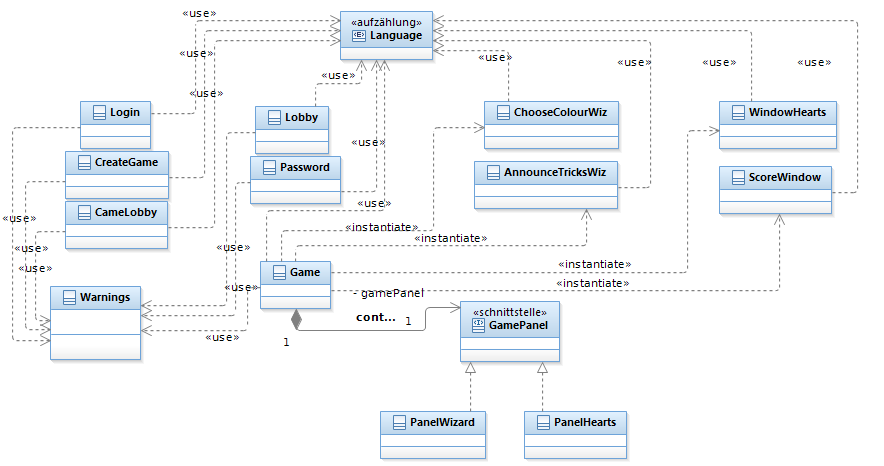
\includegraphics[width=\textwidth]{ClientView}
\textbf{Language} [Enumerator]: Language wird zur Darstellung der Sprachen Deutsch, Englisch und Bayerisch  in der View verwendet (/L350W/). \\

\textbf{Login} [implementiert Observer]: Das Login-Fenster repräsentiert den initialen Dialog zwischen Benutzer und Client.\\
In diesem Fenster kann der Benutzer seinen Namen (/F042/) und die Adresse des Servers (/F040/) eingeben. Außerdem ist über den Login die Auswahl der Sprache möglich (/F050W/). Über den Login-Button wird die Verbindung zum Server hergestellt (/F045/).\\

\textbf{Lobby} [implementiert Observer]: Dieses Fenster erzeugt die Ansicht der ServerLobby auf der Client Seite, in der die Spieler neue Spiele erzeugen oder offenen beitreten können.\\
In der Lobby werden die Benutzernamen der sich in der Lobby befindlichen Spieler(/L100/) , sowie die  offene Spiele (/L110/) angezeigt. In der Lobby konnen Chatnachrichten gesendet (/F060/) und empfangen werden (/L115/). Über Leave verlässt der Spieler das Spiel (/F090/). Über Host Game (/F080/) wird der Spieler zum CreateGame Fenster weiter geleitet und mit Join Game (/F070/) kann einem bereits erstellten Spiel beigetreten werden. \\

\textbf{CreateGame} [implementiert Observer]: Das Fenster CreateGame dient dem Benutzer zur Erstellung eines neuen Spieles.\\
Es bietet alle Komponenten um ein Regelwerk zu wählen (/F120/), einen Spielnamen festzulegen (/F122/) und das Spiel durch ein Passwort zu schützen (/F130W/). In der Spielerstellung wird ein Titelbild des ausgewählten Spiels und eine kurze Beschreibung angezeigt (/L120/, /L122/). Über Leave kehrt der Spieler in die Lobby zurück (/F124/) und mit Create wird das Spiel erstellt (/F126/).\\

\textbf{Password [implementiert Observer]}: Dieses Fenster ermöglicht die Eingabe eines Passwortes (/F140W/) um einem Passwortgeschütztem Spiel beizutreten (/F142/) oder per Leave wieder in die Lobby zurückzukehren (/F145/). \\

\textbf{GameLobby} [implementiert Observer]: Die GameLobby modelliert das Wartefenster, in dem beigetretene Spieler (/L155/) auf den Start des Spieles durch den Spielleiter warten (/F200/).\\
 Der Spielleiter kann Spieler mit dem Remove Player Button entfernen (/F180/). Über Leave kehren die Spieler in die Lobby zurück (/F170/, /F190/). Der spielinterne Chat ist ab hier verfügbar (/F160/, /L158/). \\

\textbf{Game} [implementiert Observer]: Game ist das Fenster, in welchem das eigentliche Spiel abläuft.\\
Das Game-Fenster beherbergt  der den Spielchat (/F220/, /L260/) und enthält ein GamePanel. Das GamePanel zeigt die eigenen Karten (/L190/), sowie zum Ausspielen anwählbare Karten (/F225/, /F230/), die Anzahl der Karten der Mitspieler (/L192/) und den Ablagestapel (/L194/). Nach jeder Runde wird der Punktestand  aktualisiert (/L200/). Schließen beendet das Spiel und der Spieler wird in die Lobby zurückgeleitet (F210/).\\

\textbf{GamePanel}: Das Panel ist die Komponente des Game-Fensters, welche das eigentliche Spiel darstellt.\\
Es besteht aus veschiedenen Panelobjekten, welche je nach Regelwerk auf das Spielfeld gezeichnet werden.
\textbf{OwnHand}: Stellt die Karten dar, die der Spieler auf der Hand hat. (?Zusatzlich gibt es zwei Label für den eigenen Punktestand und die zusätzlichen Angaben, wie z.B. die Stiche in Wizard?)\\
\textbf{OtherPlayer}: Zeigt die Informationen über die anderen Spieler, also den Namen, ein Symbol für die verdeckte Hand und das Label für zusätzliche Angaben. (?Ablagestapel?)\\
\textbf{DiscardPile}: Stellt einen Ablagestapel dar.\\
\textbf{DrawDeck}: Stellt einen Aufnahmestapel dar. Bei Wizard wird dort die Trumpffarbe angezeigt.\\

\textbf{Warning} [implementiert Observer]: Das Warning-Fenster zeigt dem Benutzer Fehlermeldungen bzw. Hinweise an (/L290/), (?welche vom ClientModel übergeben wurden?). \\

\textbf{ChooseColour} [implementiert Observer]: Dieses Fenster ermöglicht es Spielern eine Trumpffarbe auszuwählen (/F360/). \\

\textbf{InputNumber} [implementiert Observer]: In diesem Fenster, kann der Benutzer eine Zahl eingeben, um z.B zu Beginn einer Runde Wizards seine Stiche zu schätzen (/F370/). \\

\textbf{ChooseCards} [implementiert Observer]: In dieses Fenster wählt der Benutzer zu Beginn einer Partie Hearts, welche Karten er zu anderen Spielern weiterreichen wird (/F260/). \\

\textbf{ScoreWindow} [implementiert Observer]: Dieses Fenster zeigt den momentanen Punktestand nach jeder Runde und den Gesamtpunktestand am Ende des Spieles an (/L250/).\\

\textbf{Observer}[Interface]: Stellt das Observer-Pattern der View dar.\\
 Die GUIs nutzen die update() Methode, sobald im ClientModel notify() aufgerufen wird, um Veränderungen durchzuführen.

\subsection{Ruleset}
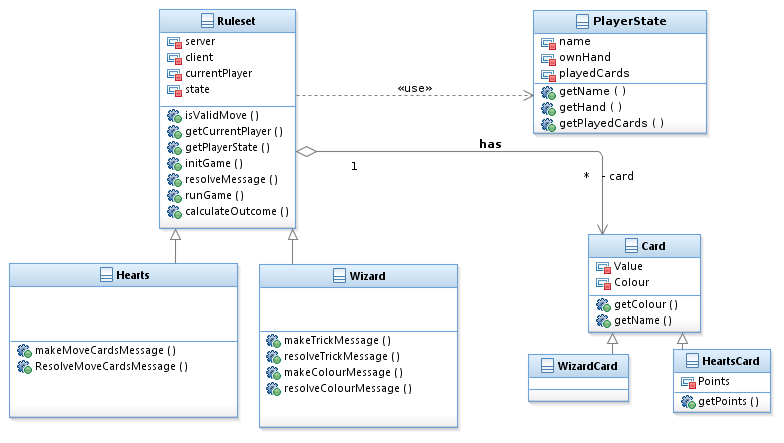
\includegraphics[width=\textwidth]{Ruleset}
\textbf{Ruleset} ist eine abstrakte Klasse, welche zu einem Spiel die Regeln und den Ablauf bestimmt (/L280/). Außerdem überprüft es, ob jeder neuer Spielzustand regelkonform ist (/L280/). Das Regelwerk wird im Client, sowie im Server instanziert. Im Server hält es Zustandsinformationen von allen Spielern, im Client jedoch nur von seinem entsprechendem Spieler (/L330/). Über resolveMessage() kann eine GameServerinstanz ein ComObjekt vom Player an das Regelwerk weiterleiten. Die Methoden runGame() und calculateOutcome() starten das Spiel bzw. ermitteln den Gewinner und Punktestand eines Spiels. \\
		\textbf{Hearts} erbt von Ruleset und erstellt das Regelwerk zum Spiel Hearts. \\
		\textbf{Wizard} erbt von Ruleset und erstellt das Regelwerk zum Spiel Wizard. \\
		\textbf{PlayerState} modelliert den Spielzustand eines Spielers, dessen Namen, Karten und Spielzug. Auch hält die Klasse die dazugehörigen getter Methoden bereit. PlayerState wird von Instanzen des Ruleset verwendet. \\
		\textbf{Card} ist eine abstrakte Klasse und repräsentiert eine Karte. Jede Karte besitzt als Attribute einen Wert und eine Farbe. \\
		\textbf{HeartsCard} repräsentiert eine Karte aus dem Spiel Hearts. \\
		\textbf{WizardCard} repräsentiert eine Karte aus dem Spiel Wizard.

\subsection{ComObjects}
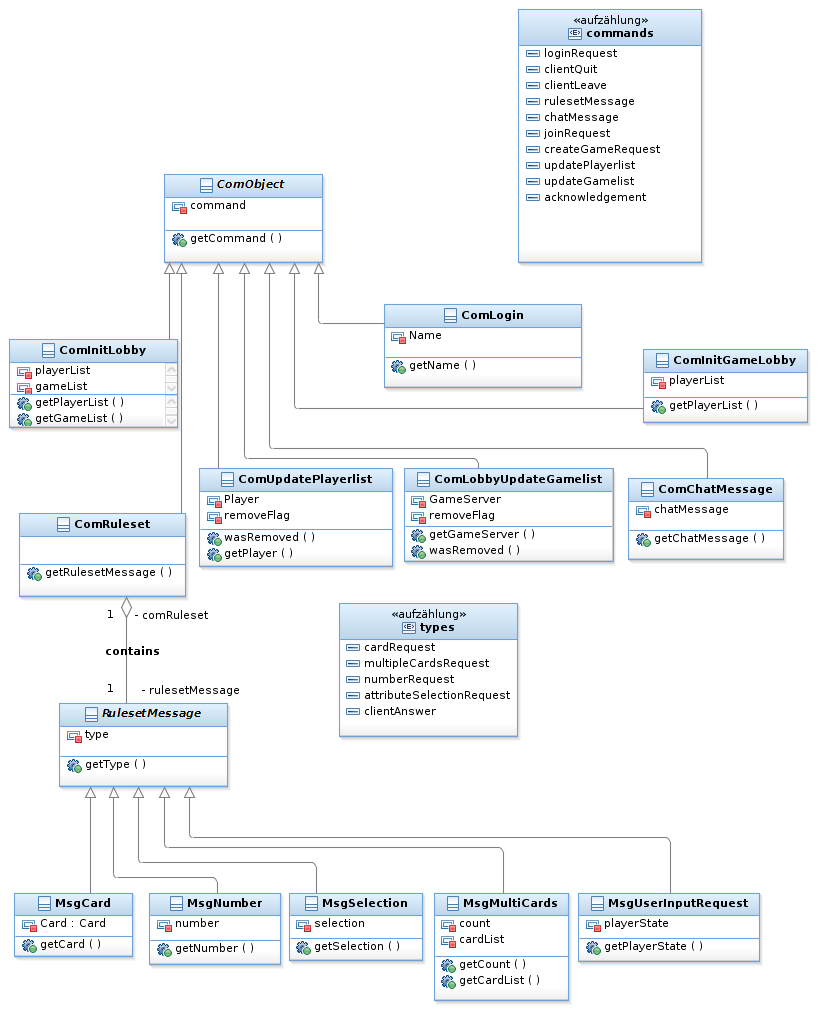
\includegraphics[width=\textwidth]{ComDiagram}
\textbf{ComObject} Grundlegende ComObject Klasse von der alle anderen erben.\\
		\textbf{ComInitLobby} synchronisiert den Client mit der Lobby, wenn er sich mit dem Server verbindet oder nach einem Spiel in die Lobby zurückkehrt. \\
		\textbf{ComUpdatePlayerList} \\
		\textbf{ComLogin} Nachricht, die beim Login an den Server gesendet wird.\\
		\textbf{ComLobbyUpdateGameList} aktualisiert die Spielerliste in der Lobby und Spiellobby.\\
		\textbf{ComInitGameLobby} liefert die Liste der Spieler, die sich bereits beim Betreten der Spiellobby darin befinden. \\
		\textbf{ComChatMessage} Das ComObjekt einer Chatnachricht. Liefert die Chatnachricht in Form eines Strings.\\
		\textbf{ComRuleset} Grundlegende Nachricht eines Regelwerkaufrufes. Trägt eine verfeinerte Nachricht mit weiteren Informationen.\\
		\textbf{RulesetMessage} vererbt an alle Nachrichten für das Regelwerk.\\
		\textbf{MsgCard} beinhaltet die ausgespielte Karte eines Spielers.\\
		\textbf{MsgNumber} gibt eine Nummer zurück, welche für die Stichansage in Wizard verwendet werden kann.\\
		\textbf{MsgSelection} gibt eine Farbe zurück, welche für die Ansage der Trumpfarbe in Wizard verwendet werden kann.\\
		\textbf{MsgMultiCards} liefert mehrere Karten zum Tausch für das Regelwerk Hearts. \\
		\textbf{MsgUserInputRequest} wird dem Client gesendet, um den aktuellen Zug anzusagen.\\
		\textbf{enum commands}  Enumerator, der ComObjekte ihre Kommandos zuweist. \\
		\textbf{enum types} Enumerator zur eindeutigen Identifizierung von Regelwerknachrichten.

\ \\

\section{Sequenzdiagramme}
	\subsection{Spielstart}
		Mr. Blue, Mr. White und Mr. Pink befinden sich in der Lobby. \\
		Mr. Blue klickt auf 'New Game' und wird ins Erstellungsfenster geschickt. \\
		Er nimmt die nötigen Einstellungen vor (z.B. Wizard auswählen, Name setzen) und drückt auf 'Create'. Er wird ins Wartefenster weitergeleitet.\\
		Mr. Pink und Mr. White wählen Mr. Blues Spiel in der Lobby aus und drücken auf 'Join'. Sie werden an die Passwortabfrage geschickt.\\
		Sie geben das Passwort ein und werden ans Wartefenster geschickt.\\
		Die Mindestanzahl von drei ist erreicht. Mr. Blue drückt auf 'Start Game'.\\
		Mr. Blue, Mr. Pink und Mr. White werden ins Spiel geschickt. Das Spiel startet.\\

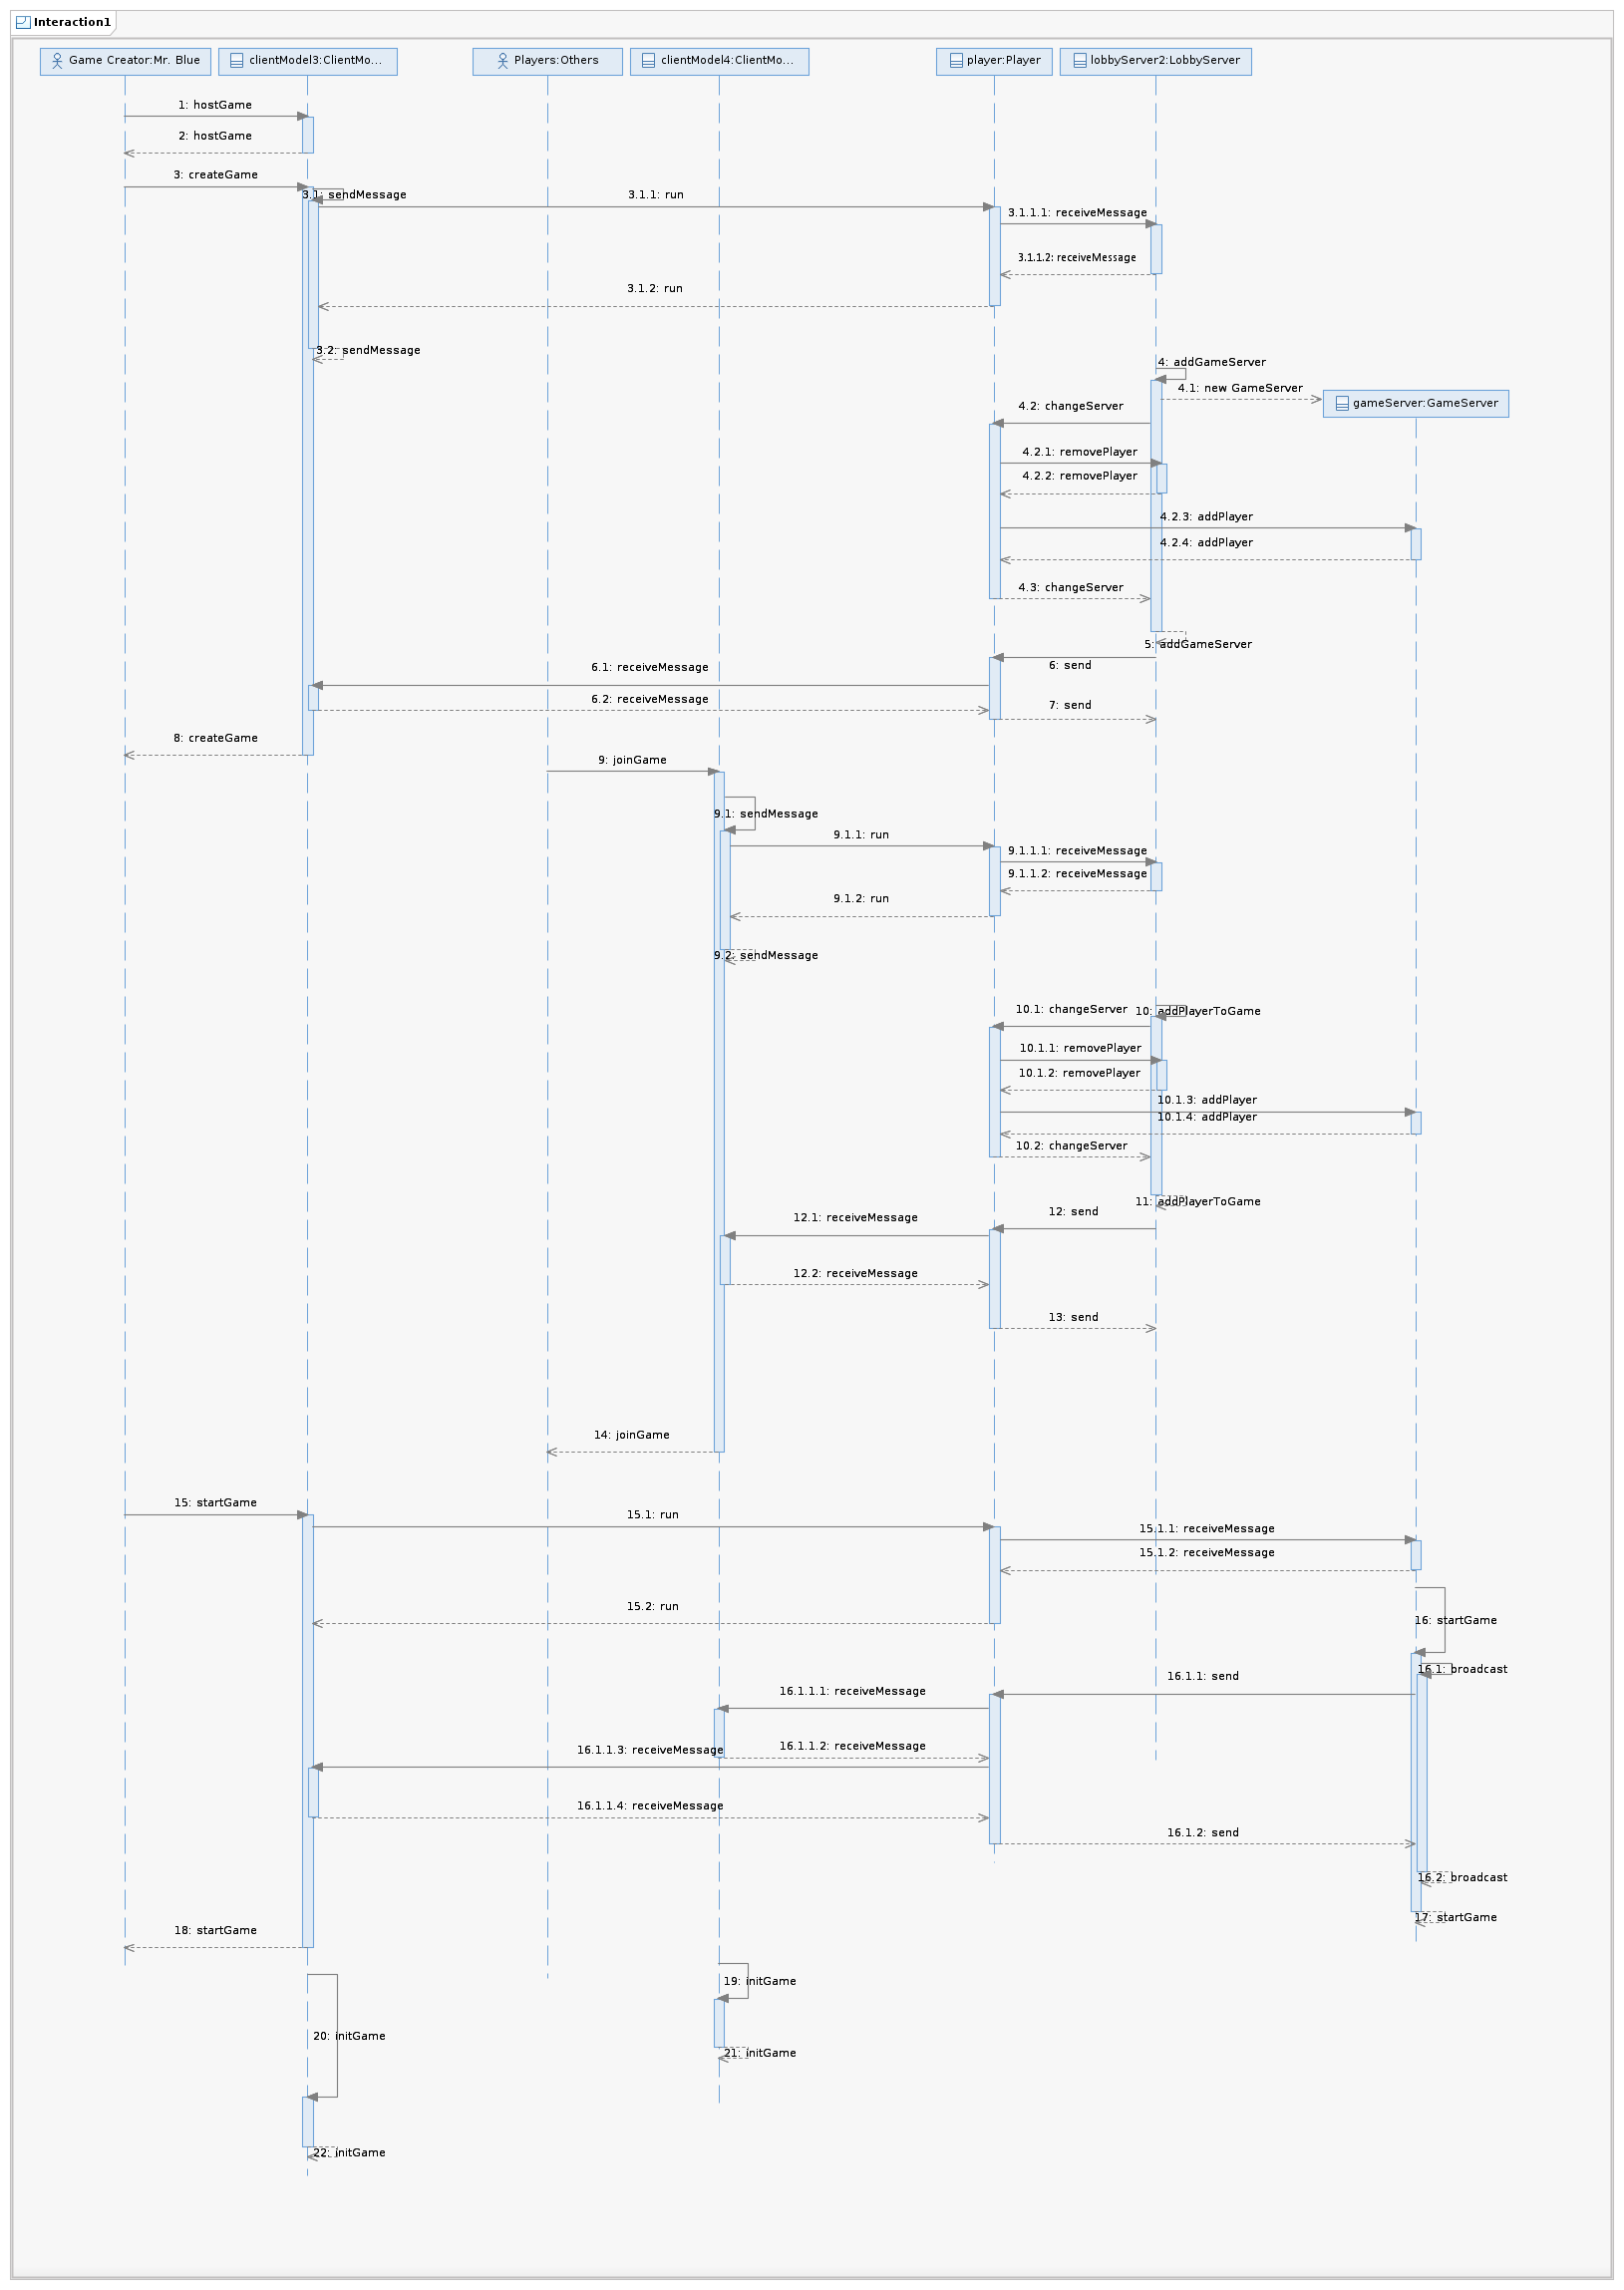
\includegraphics[width=\textwidth]{Entwurf_CreateGame}

\subsection{Spielzug}
		Aufgabe: Ein Spieler ist im Spiel Wizard an der Reihe und spielt eine Karte aus.
		Das Diagramm endet, sobald der Spielzug auf allen Clients sichtbar
		geworden ist und der nächste Spieler seinen Zug machen kann.\\
		\ \\
		Mr. Blue, Mr. White und Mr. Pink sind im Spiel Wizard. \\
		Mr. Blue ist an der Reihe, wählt eine Karte durch einmaliges Anklicken aus und spielt sie durch ein weiteres Anklicken.\\
		Der Zug wird auf Regelkonformität überprüft.\\
		Er ist nicht regelwidrig, also wird die gepielte Karte über den Server verschickt und bei Mr. Blue, Mr. Pink und Mr. White auf dem Ablagestapel angezeigt. \\
		Es wird überprüft, wer als nächstes dran ist.\\
		Der nächste Spieler ist am Zug. \\

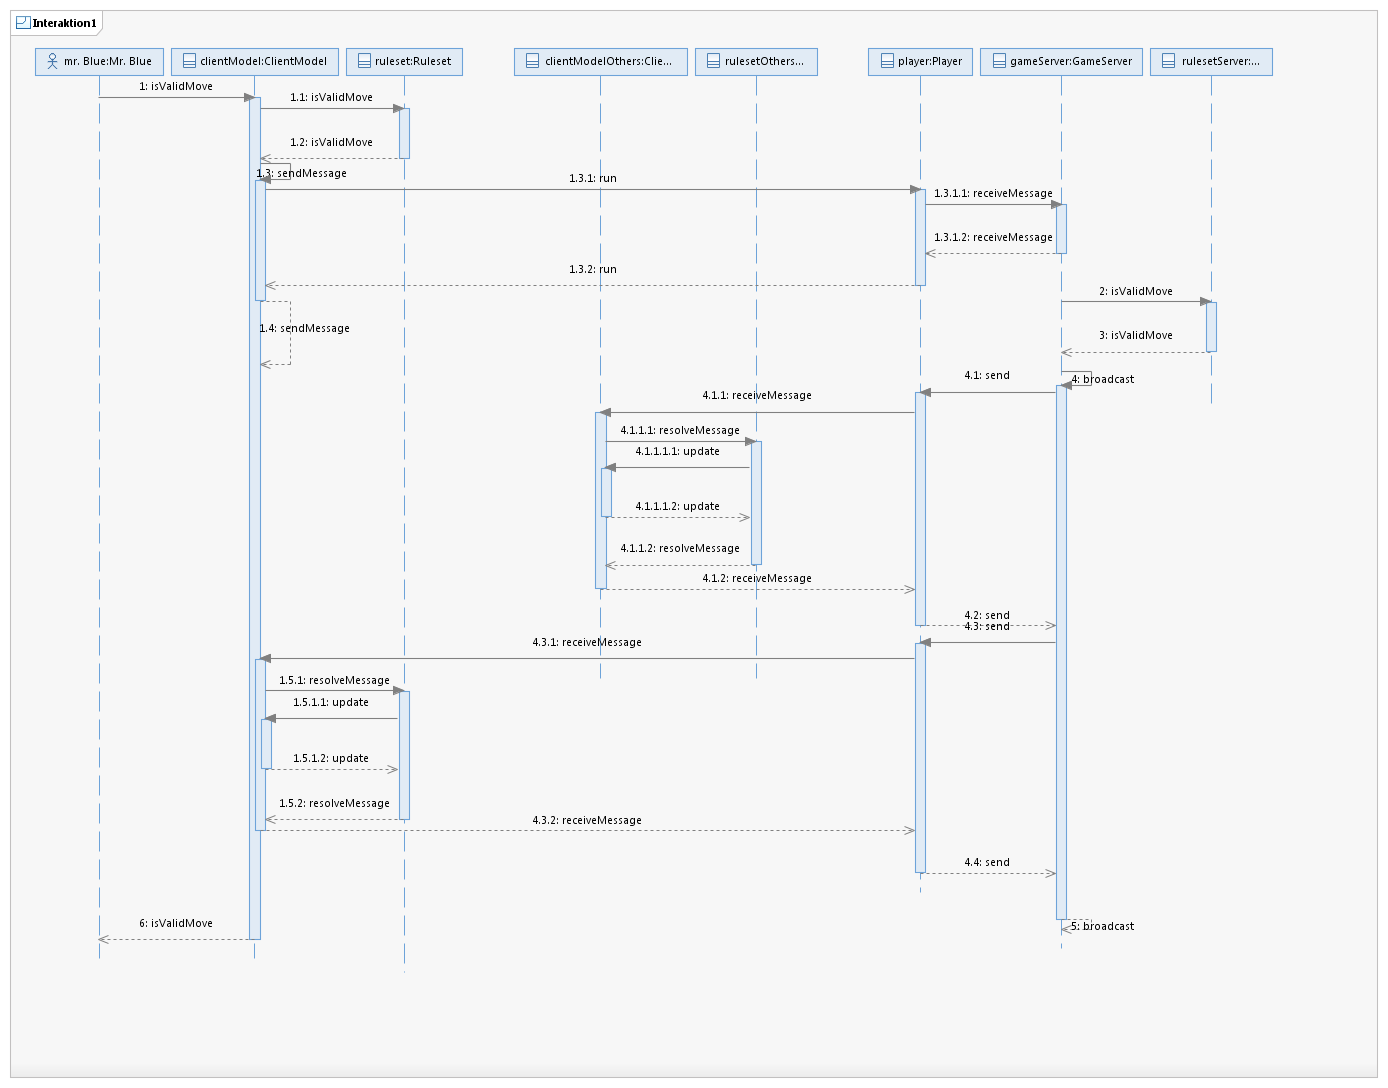
\includegraphics[width=\textwidth]{Entwurf_PlayCard}
		
\end{document}
